% 115-82(115쪽) — 한 변의 길이가 6인 정삼각형에서 각 변의 중점을 이어 만든 가운데 정삼각형을
% 오려 낸 1회 시행 그림(원문 「오른쪽 그림」). 스캔 화질이 낮아 TikZ 로 다시 그림.
% 원문처럼 1회 시행까지만 그리고(남은 3개의 작은 정삼각형만 색칠), 라벨은 원문에 있는 「6」 하나뿐이다.
% 15회 시행 후 남은 넓이(답)가 그림에서 읽히지 않게 넓이·비율은 적지 않는다.
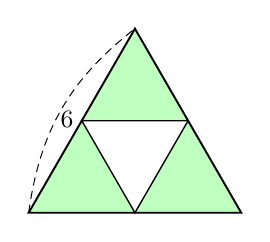
\begin{tikzpicture}[x=0.45cm, y=0.45cm, line width=0.5pt]
  \fill[green!25] (0,0) -- (3,0) -- (1.5,2.598) -- cycle;
  \fill[green!25] (3,0) -- (6,0) -- (4.5,2.598) -- cycle;
  \fill[green!25] (1.5,2.598) -- (4.5,2.598) -- (3,5.196) -- cycle;
  % 오려 낸 가운데 정삼각형(각 변의 중점을 이은 것)
  \draw (1.5,2.598) -- (4.5,2.598) -- (3,0) -- cycle;
  \draw[line width=0.7pt] (0,0) -- (6,0) -- (3,5.196) -- cycle;
  \draw[densely dashed, line width=0.35pt] (0,0) to[bend left=22] (3,5.196);
  \node[font=\small] at (1.08,2.62) {$6$};
\end{tikzpicture}
